\documentclass[tikz]{standalone}

\usepackage{amsmath}

\renewcommand{\vec}[1]{\boldsymbol{#1}}

\tikzset{>=latex}
\begin{document}
\begin{tikzpicture}
  \node[coordinate] (A) at (3.55,4.75) {};
  \node[coordinate] (P) at (6.3,1.95) {};
  \node[coordinate] (fa_init) at (1.55,6.7864) {};
  \node[coordinate] (fa_final) at (3.45,4.8518) {};
  \node[coordinate] (r_init) at (8.3,-0.0864) {};
  \node[coordinate] (r_final) at (6.4,1.8482) {};
  
  \node[anchor=south west,inner sep=0] at (0,0) {
    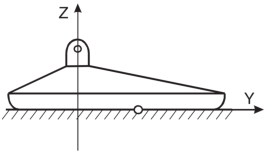
\includegraphics[width=\textwidth]{zmp_foot_y_example_figure}};

  \node[left=5, below=1, font=\sffamily] at (A) {\Large A};
  \node[right=8, above=1, font=\sffamily] at (P) {\Large P};
  
  \draw[dashed, very thick,line width=1mm, red] (A) -- (P);
  \draw[->=stealth, very thick, line width=1mm, black]  (fa_init) -- (fa_final) node[font=\sffamily, left=25, above=2] {\Large $\vec{F}_A$};
  \draw[->=stealth, very thick, line width=1mm, black]  (r_init) -- (r_final) node[font=\sffamily, right=7, below=12] {\Large $\vec{R}$};
\end{tikzpicture}
\end{document}
